\section{Результаты измерений и обработка данных}

\subsection{Спектры прямоугольных импульсов}

Выполним указанный в инструкциях тест спектра прямоугольных импульсов: Изменяя параметры спектра, такие как частота и ширина сигналов, сохраним четыре различных картины спектра (см. рис. 4-5).

\begin{figure}{\textwidth}
\begin{subfigure}{.5\textwidth}
    \centering
    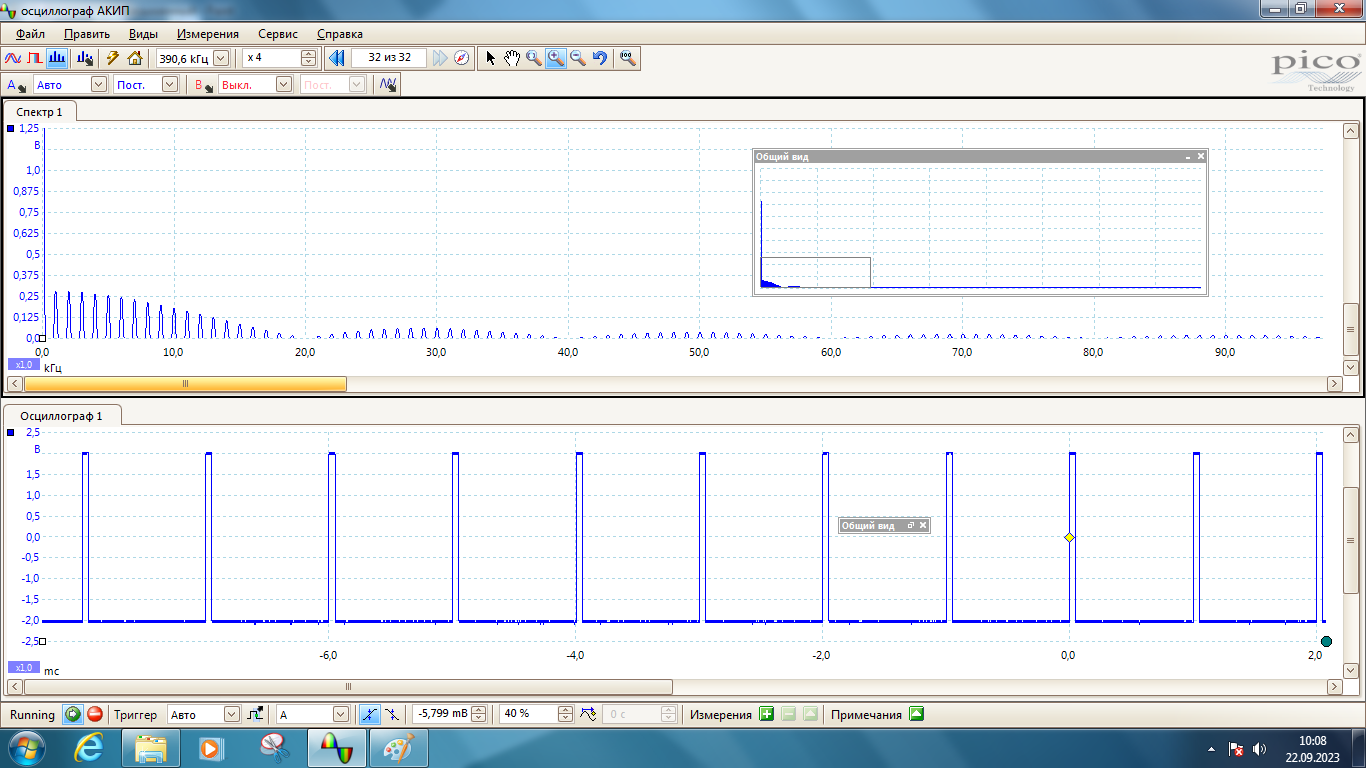
\includegraphics[width=\linewidth]{1000_50.png}
    \caption{$\nu$ = 1 кГц, $\tau$ = 50 мкс}
    \label{fig:table1}
\end{subfigure}%
\begin{subfigure}{.5\textwidth}
    \centering
    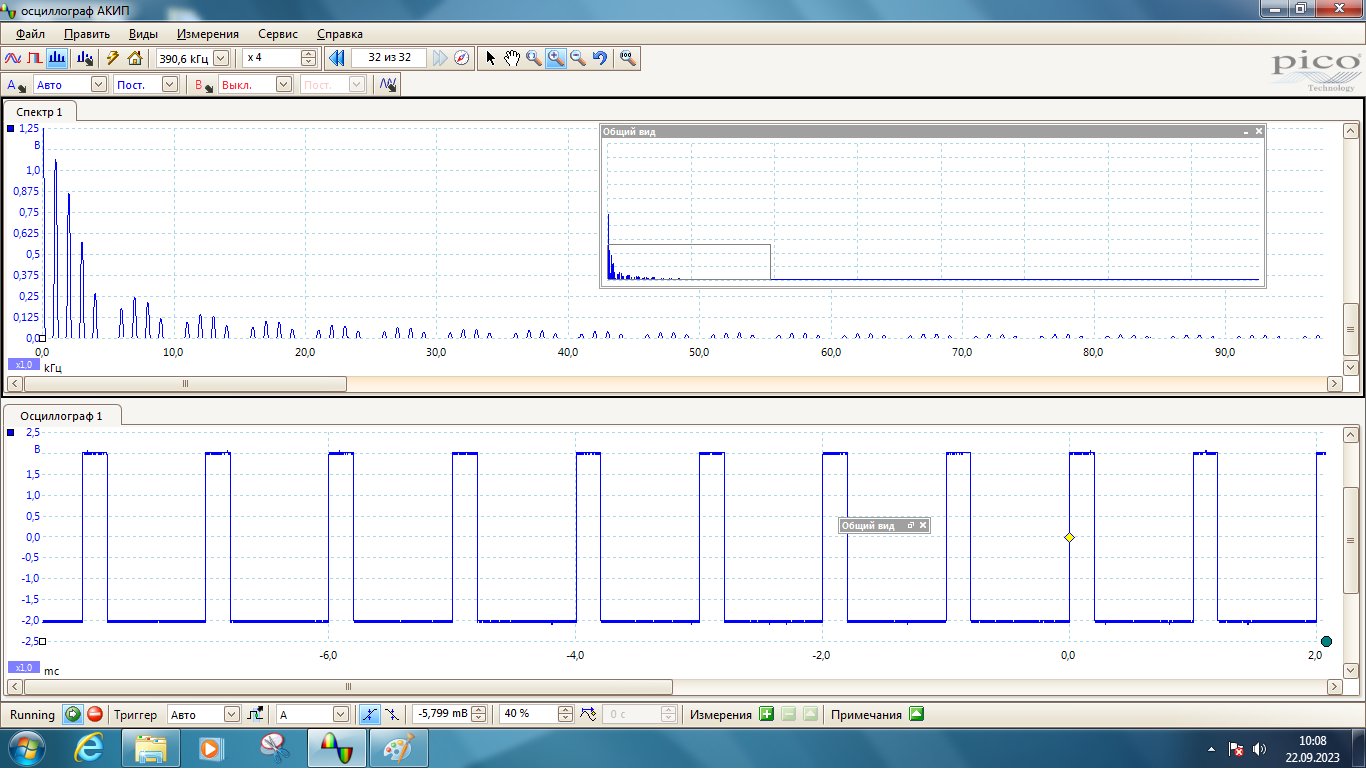
\includegraphics[width=\linewidth]{1000_200.png}
    \caption{$\nu$ = 1 кГц, $\tau$ = 200 мкс}
    \label{fig:table1}
\end{subfigure}
\caption{}
\end{figure}

\begin{figure}{\textwidth}
\begin{subfigure}{.5\textwidth}
    \centering
    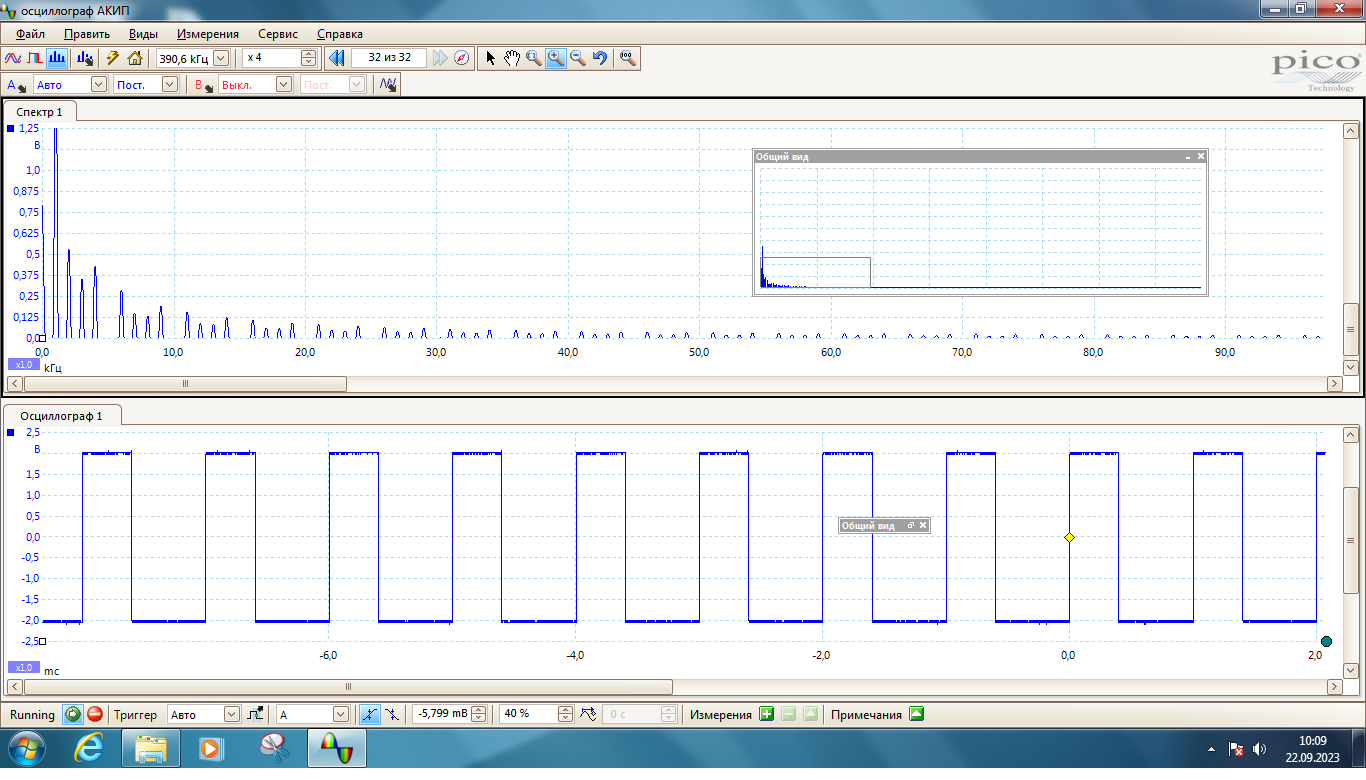
\includegraphics[width=\linewidth]{1000_400.png}
    \caption{\nu = 1 кГц, \tau = 400 мкс}
    \label{fig:table1}
\end{subfigure}%
\begin{subfigure}{.5\textwidth}
    \centering
    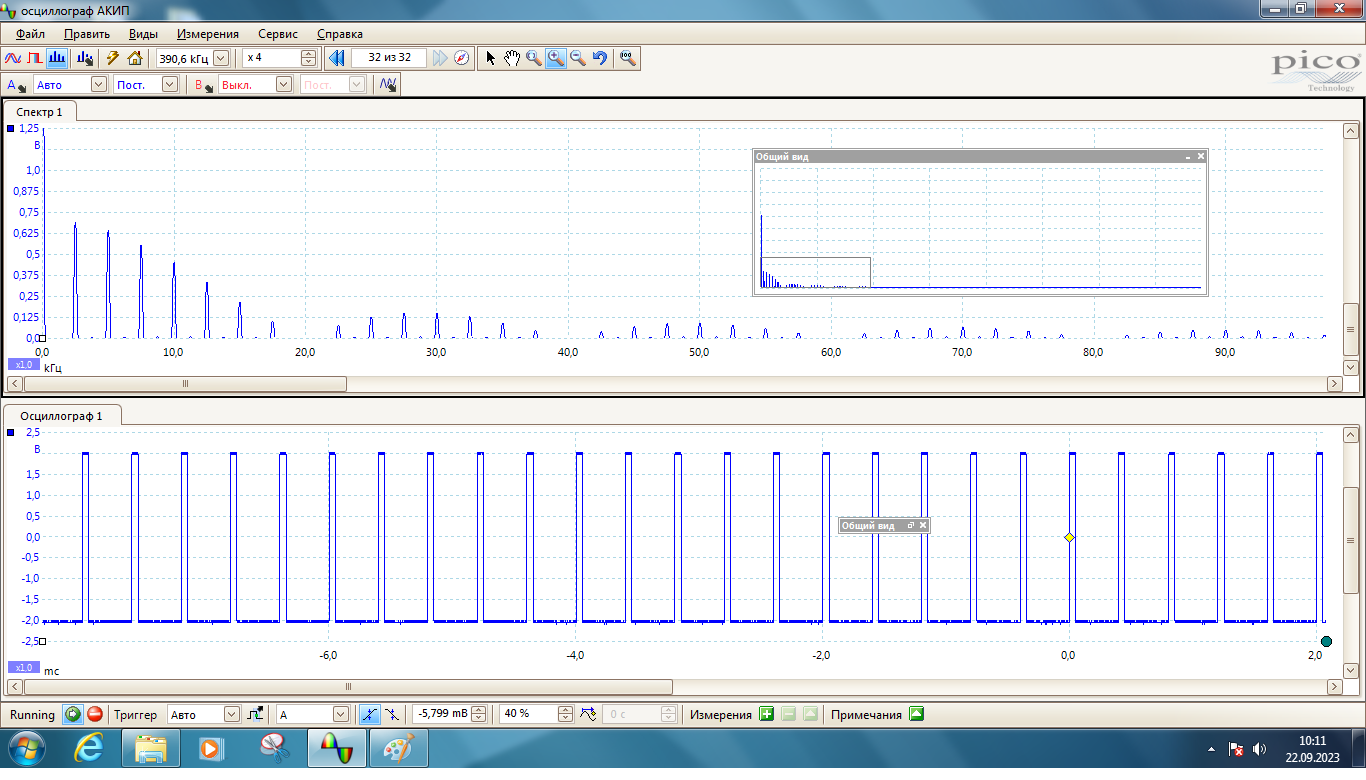
\includegraphics[width=\linewidth]{2500_50.png}
    \caption{\nu = 2,5 кГц, \tau = 50 мкс}
    \label{fig:table1}
\end{subfigure}
\end{figure}

Заметим, что при возрастании $ \tau $ вдвое, ширина спектра уменьшается в 2 раза и в 2 раза возрастает амплитуда спектра.

При увеличении $ f_{повт} = 1/T $ в 2 раза, ширина спектра и $ \delta \nu $ -- частота 1-й гармоники --  увеличивается во столько же раз.

Зафиксируем частоту в 1 кГц и ширину импульса в 50 мкс и считаем данные о гармониках сигнала.
Заполняем таблицу для данных гармоник этих импульсов (см. рис.6)

\begin{figure}[h]
    \centering
    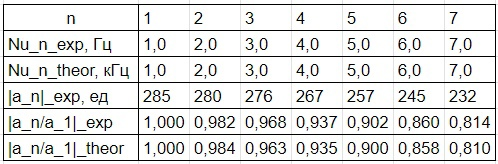
\includegraphics[width=12.5cm, height=4cm]{P_7.jpg}
    \caption{Данные гармоник сигнала}
    \label{fig:table1}
\end{figure}

Далее изменяем $\tau$ и считывем при этом полную ширину спектра сигнала$\Delta \nu$
\begin{figure}[h]
    \centering
    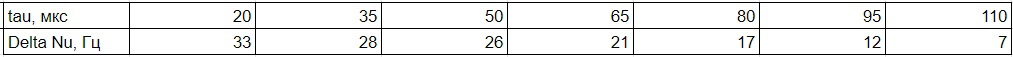
\includegraphics[width=12.5cm, height=1cm]{P_8_table.jpg}
    \caption{Данные о промежутке $\Delta \nu$ при разных $\tau$}
    \label{fig:table1}
\end{figure}

Далее замеряем расстояния между пиками T и разницу между частотами этих пиков $\delta \nu$
\begin{figure}[h]
    \centering
    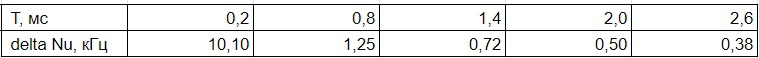
\includegraphics[width=12.5cm, height=1cm]{P_9_table.jpg}
    \caption{Данные разности частот $\delta \nu$}
    \label{fig:table1}
\end{figure}

На основании полученных из двух предыдущих пунктов данных строим соответствующие им графики:
\begin{figure}{\textwidth}
\begin{subfigure}{.5\textwidth}
    \centering
    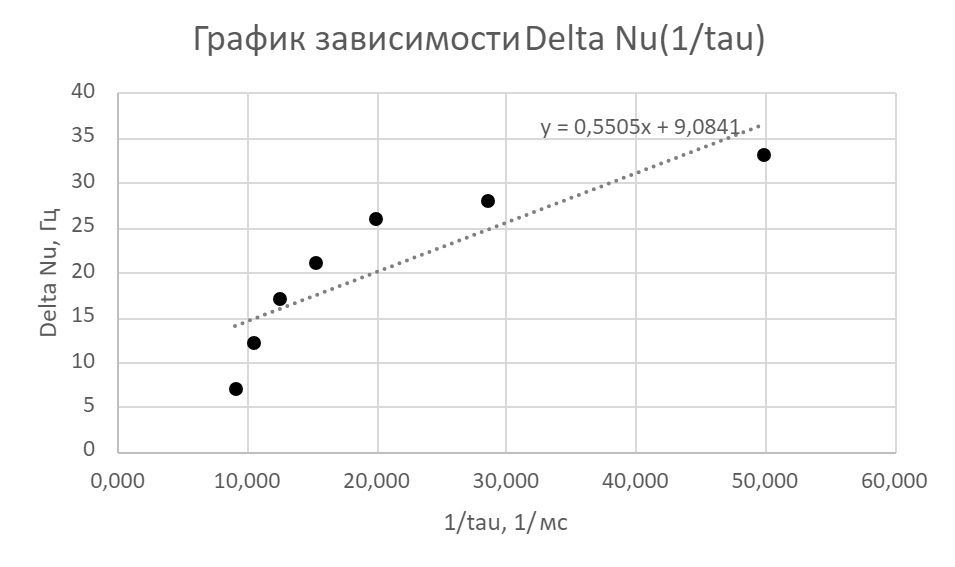
\includegraphics[width=\linewidth]{P_8.jpg}
    \label{fig:table1}
\end{subfigure}%
\begin{subfigure}{.5\textwidth}
    \centering
    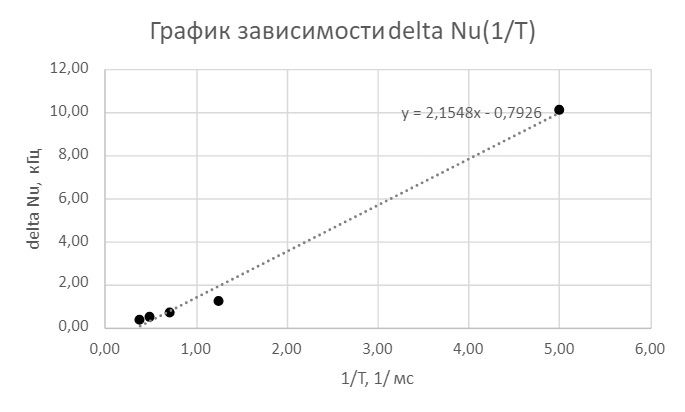
\includegraphics[width=\linewidth]{P_9.jpg}
    \label{fig:table1}
\end{subfigure}
\caption{}
\end{figure}

\subsection{Спектры цугов гармонических  колебаний}

Переводим генератор в режим гармонических колебаний и также выбираем четыре комбинации значений $\nu_0$, T и N для изучения. Данные с осциллографа при этих комбинациях представлены в таблице на рис. 10, а также на снимках экрана на рис. 11-12:
\begin{figure}[h]
    \centering
    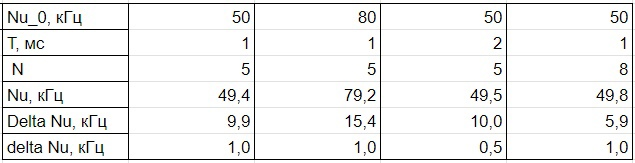
\includegraphics[width=13cm, height=3.5cm]{P_14.jpg}
    \caption{Данные гармонических колебаний}
    \label{fig:table1}
\end{figure}

\begin{figure}{\textwidth}
\begin{subfigure}{.5\textwidth}
    \centering
    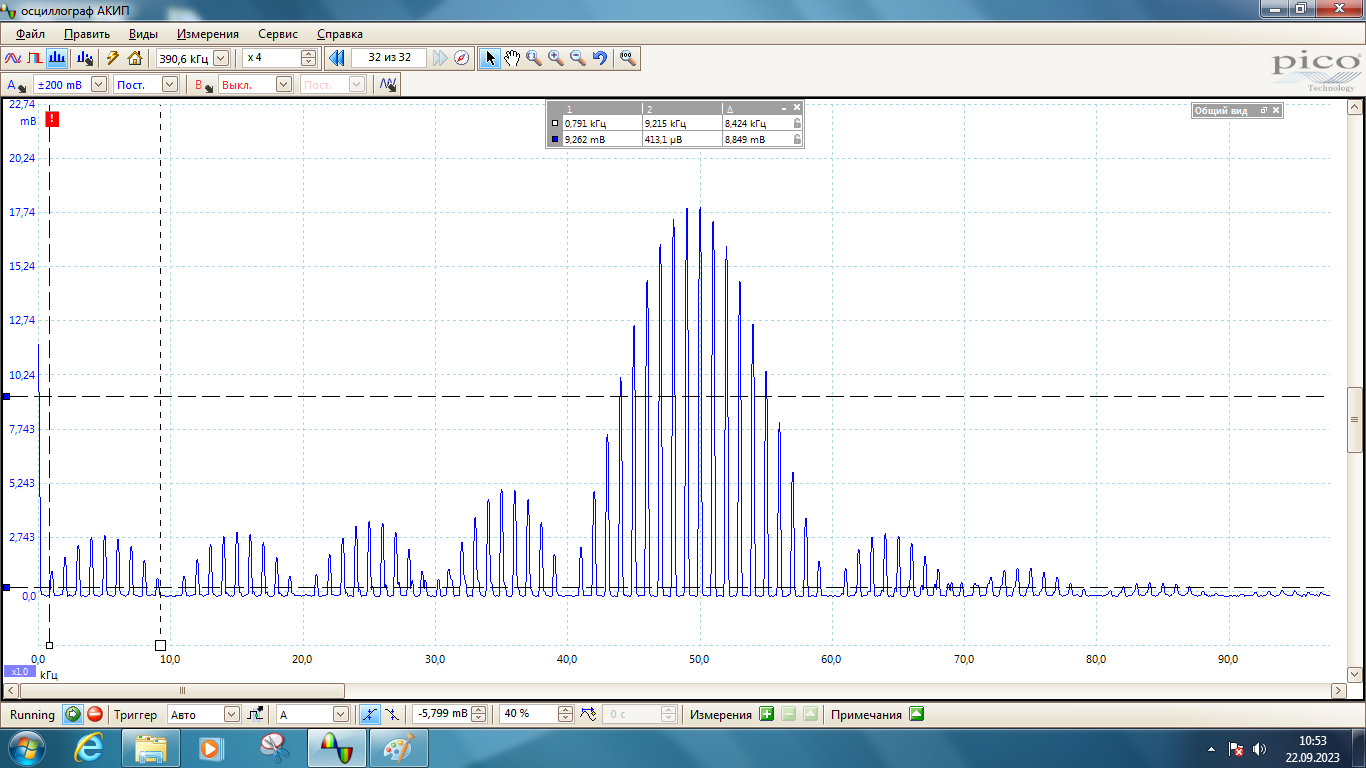
\includegraphics[width=\linewidth]{50_1_5.png}
    \caption{\nu = 50 Гц, T = 1 мс, N = 5}
    \label{fig:table1}
\end{subfigure}%
\begin{subfigure}{.5\textwidth}
    \centering
    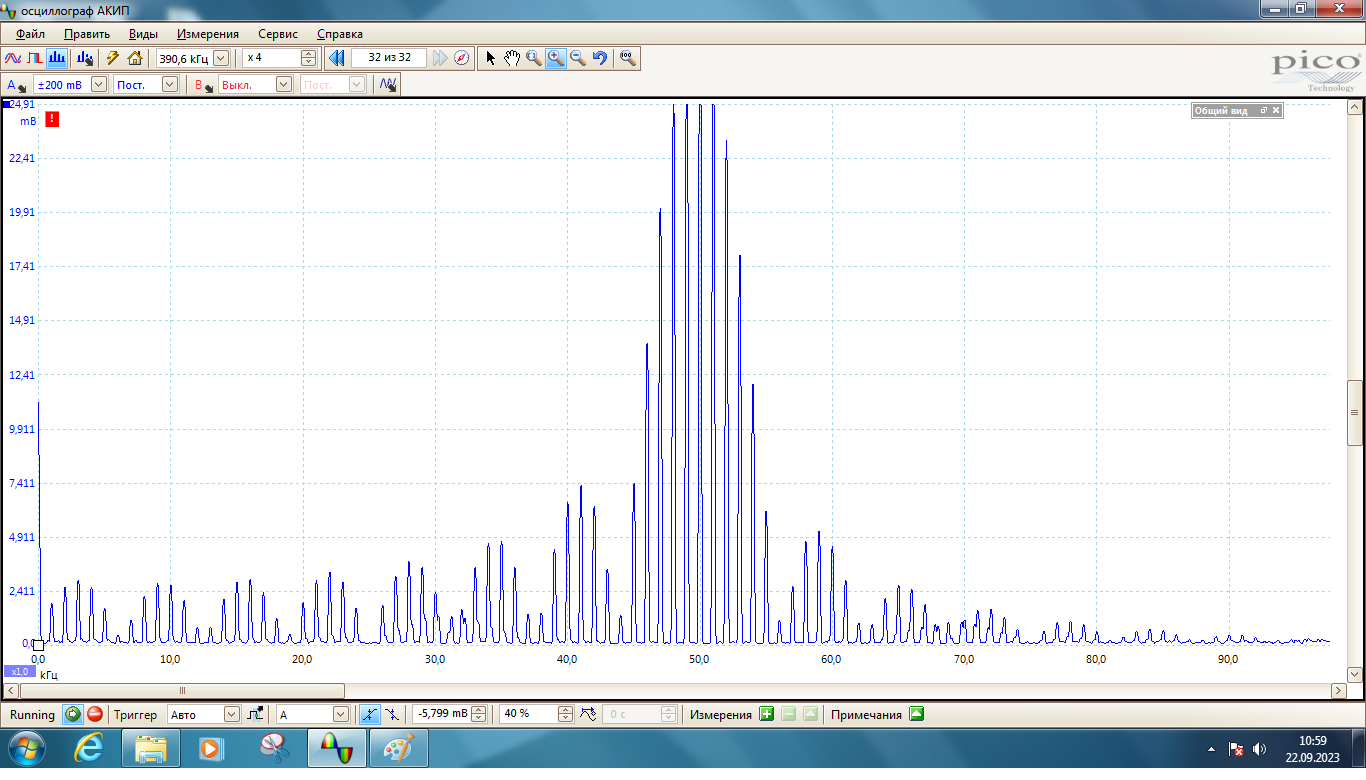
\includegraphics[width=\linewidth]{50_1_8.png}
    \caption{\nu = 50 Гц, T = 1 мс, N = 8}
    \label{fig:table1}
\end{subfigure}
\caption{}
\end{figure}

\begin{figure}{\textwidth}
\begin{subfigure}{.5\textwidth}
    \centering
    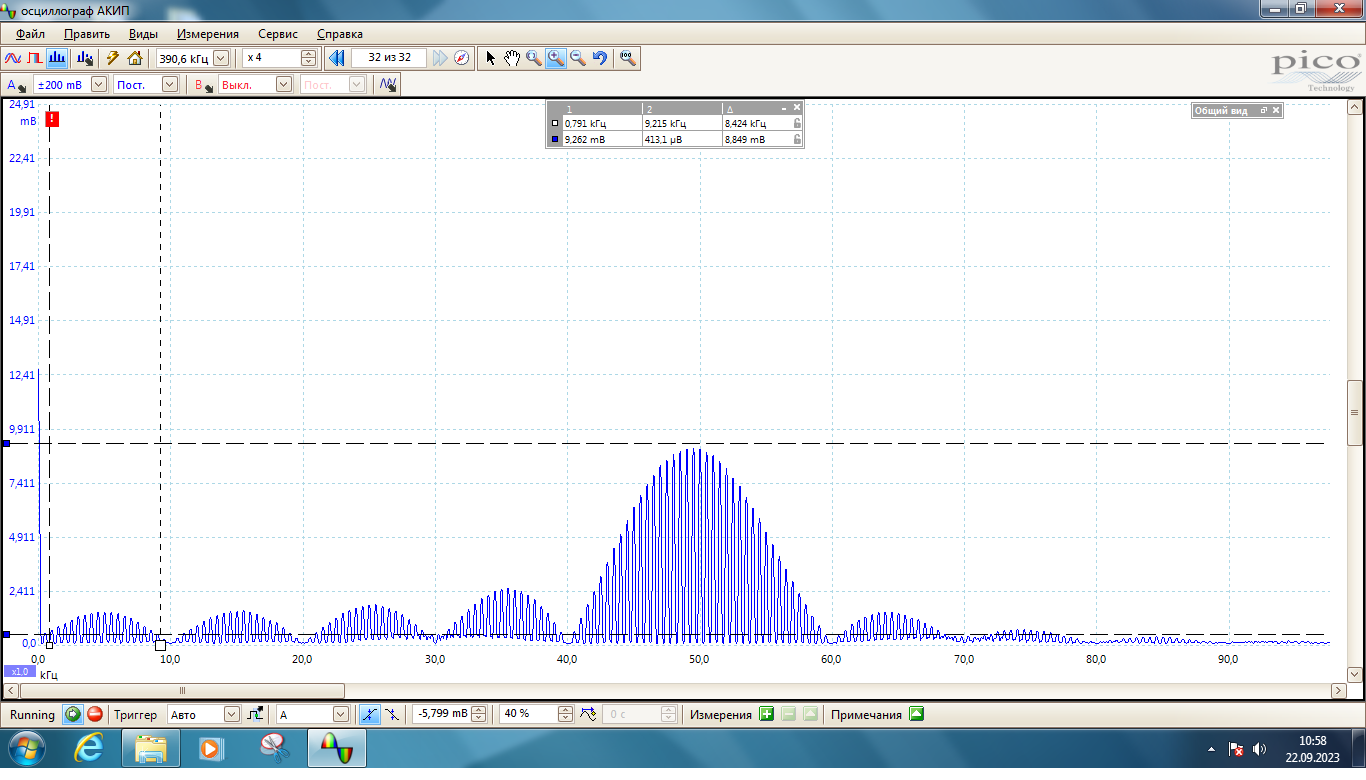
\includegraphics[width=\linewidth]{50_2_5.png}
    \caption{\nu = 50 Гц, T = 2 мс, N = 5}
    \label{fig:table1}
\end{subfigure}%
\begin{subfigure}{.5\textwidth}
    \centering
    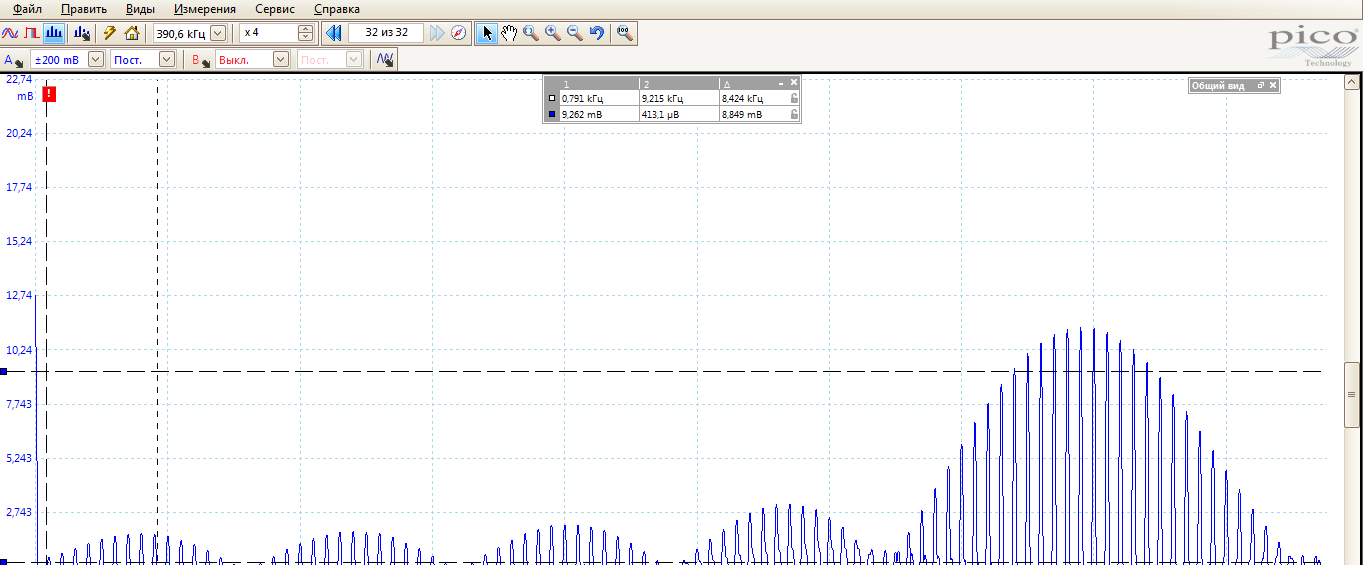
\includegraphics[width=\linewidth]{80_1_5.png}
    \caption{\nu = 80 Гц, T = 1 мс, N = 5}
    \label{fig:table1}
\end{subfigure}
\caption{}
\end{figure}

\subsection{Спектры АМ-сигналов}
Переводим генератор и осциллограф в режим генерации и измерения амплитудно-моделированного сигнала. Сначала выставляем рекомендуемые параметры: $\nu_0 = 50$ кГц, $\nu_{mod} = 2$ кГц, глубина модуляции m = 0,5. При помощи режима курсорного измерения в осциллографе измеряем $A_{max}$ = 1,51 В и $A_{min}$ = 0,51 В. Проверяем справедливость равенства: $m = \frac{A_{max} - A_{min}}{A_{max} + A{min}} = 0,5$.
После этого снимаем зависимость отношений амплитуд боковых и основных спектральных линий в зависимости от глубины модуляции. Результаты записываем в таблицу, представленную на рис.13, а также строим по ней график, представленный на рис.14.
\begin{figure}[h]
    \centering
    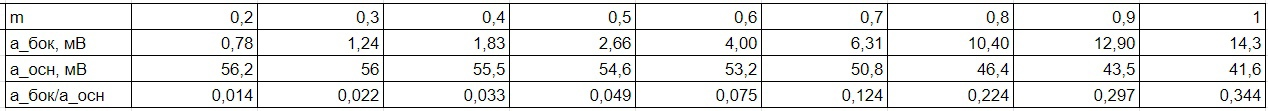
\includegraphics[width=14cm, height=2cm]{P_22.jpg}
    \caption{Результаты измерений амплитудно-моделированных сигналов}
    \label{fig:table1}
\end{figure}
\begin{figure}[h]
    \centering
    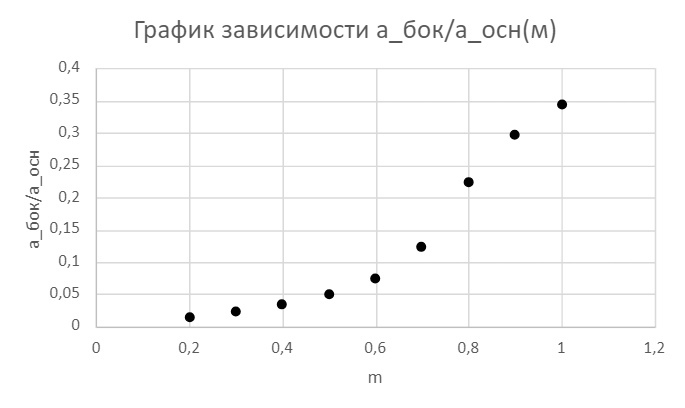
\includegraphics[width=13cm, height=7.5cm]{P_23.jpg}
    \caption{}
    \label{fig:table1}
\end{figure}
